\documentclass[10pt,noamssymb,svgnames]{beamer}
\usetheme{CambridgeUS}

\beamertemplatenavigationsymbolsempty
\usepackage{bm}
\usepackage{amsmath}
\usepackage{amssymb}
\usepackage{booktabs}
\usepackage{ragged2e}
\usepackage[vlined]{algorithm2e}
\usepackage[absolute,overlay]{textpos}
\usepackage{tikz}
\usetikzlibrary{shapes.geometric,arrows}

\tikzset{onslide/.code args={<#1>#2}{%
  \only<#1>{\pgfkeysalso{#2}} % \pgfkeysalso doesn't change the path
}}
\tikzset{temporal/.code args={<#1>#2#3#4}{%
  \temporal<#1>{\pgfkeysalso{#2}}{\pgfkeysalso{#3}}{\pgfkeysalso{#4}} % \pgfkeysalso doesn't change the path
}}

\usepackage{hyperref}
\hypersetup{colorlinks=true,urlcolor=cyan,linkcolor=}

\definecolor{CyanBlueAzure}{HTML}{4B8BBE} % light blue
\definecolor{LapisLazuli}{HTML}{306998} % dark blue

% BEAMER CONFIGURATION ---------------------------------------------------------
\newcommand<>{\blue}[1]{{\color#2{blue}#1}}
\setbeamerfont{block title}{size=\normalsize}
\setbeamerfont{block body}{size=\scriptsize}
\setbeamertemplate{mini frames}{}

%\setbeamercolor{sectiontitle}{fg=black}
% \setbeamercolor{part title}{fg=black}
% \setbeamercolor{progress bar}{fg=CyanBlueAzure}
% \setbeamercolor{progress bar in head/foot}{fg=LapisLazuli,bg=CyanBlueAzure}
% \setbeamercolor{progress bar in section page}{fg=LapisLazuli,bg=CyanBlueAzure}
% \setbeamercolor{frametitle}{bg=black!75!white}

% Configure progress bars
% \metroset{progressbar=frametitle}
% \makeatletter
% \setlength{\metropolis@progressonsectionpage@linewidth}{1pt}
% \setlength{\metropolis@progressinheadfoot@linewidth}{2pt}
% \makeatother

% Blank footnote
\newcommand\blfootnote[1]{%
  \begingroup
  \renewcommand\thefootnote{}\footnote{#1}%
  \addtocounter{footnote}{-1}%
  \endgroup
}

\bibliographystyle{ans}
\setbeamertemplate{bibliography item}{\insertbiblabel}

\newcommand{\highlight}[1]{%
  \colorbox{yellow!20}{$\displaystyle#1$}}

\newcommand{\vect}[1]{\mathbf{#1}} % vectors and matrices

% TIKZ CONFIGURATION -----------------------------------------------------------
\tikzstyle{start} = [rectangle, draw, fill=green!20, rounded corners=3mm,
  centered, minimum height=1em]
\tikzstyle{end} = [rectangle, draw, fill=red!20, rounded corners=3mm,
  centered, minimum height=1em]
\tikzstyle{process} = [rectangle, draw, fill=yellow!20, text width=8em, text
  centered, minimum height=1em]
\tikzstyle{decision} = [diamond, draw, fill=gray!20, text width=5em, text badly centered,
  inner sep=0pt]
\tikzstyle{line} = [draw, -latex', thick]

%%---------------------------------------------------------------------------%%
\title{OpenMC Workshop}
\subtitle{Depletion Briefer}
\author{ANS Student Conference}
%\institute{Argonne National Laboratory}
\date{April 13, 2023}
\titlegraphic{\includegraphics[height=0.75cm]{../images/openmc_logo.png}}

%%---------------------------------------------------------------------------%%
\begin{document}

\maketitle

\begin{frame}{Depletion}
  \begin{columns}
    \column{0.6\textwidth}
    \begin{itemize}
      \item What happens when you turn the reactor on? Atoms split; short-lived products decay.
      \item We calculate $k$ over time producing power
      \item Lets us know nuclide inventories, can calculate critical boron concentration, etc.
    \end{itemize}
    \centering
    \includegraphics[width=0.7\linewidth]{../images/fission.jpg}
  \footnotetext{Image (L): \url{https://www.open.edu/openlearn/mod/oucontent/view.php?id=26801&section=3.3}}
  \footnotetext{Image (R): \url{https://commons.wikimedia.org/wiki/File:Table_isotopes_en.svg}}
    \column{0.4\textwidth}
    \includegraphics[width=\linewidth]{../images/table_isotopes.pdf}
  \end{columns}
\end{frame}

\begin{frame}{Depletion}
  \begin{equation*}
    \begin{aligned} \frac{dN_i(t)}{dt} = &\sum\limits_j
      \underbrace{\left [ \underbrace{f_{j \rightarrow i} \color<2>{blue}{\int_0^\infty dE \;
      \sigma_j (E, t) \phi(E,t)}}_\text{nuclear reactions} +
      \underbrace{\lambda_{j\rightarrow i}}_\text{decay} \right ]
      N_j(t)}_{\text{Production of nuclide }i\text{ from nuclide }j} \\
      &- \underbrace{\left [\underbrace{\color<2>{blue}{\int_0^\infty dE \; \sigma_i
      (E,t) \phi(E,t)}}_\text{nuclear reactions} +
      \underbrace{\sum\limits_j \lambda_{i\rightarrow j}}_\text{decay} \right ]
      N_i(t)}_{\text{Loss of nuclide }i} \end{aligned}
    \end{equation*}
    \center
    OpenMC calculates the integrals involving flux!
\end{frame}

\begin{frame}{Depletion as a system of ODEs}
  \begin{equation*}
    \label{eq:depletion-matrix-t}
    \frac{d\vect{n}}{dt} = \vect{A}(\vect{n},t)\vect{n}, \quad \vect{n}(0) =
    \vect{n}_0
  \end{equation*}
  where
  \begin{equation*}
  \vect{n} = \begin{pmatrix} N_1 \\ N_2 \\ \vdots \\ N_n \end{pmatrix}, \quad
  \vect{n}_0 = \begin{pmatrix} N_{1,0} \\ N_{2,0} \\ \vdots \\ N_{n,0} \end{pmatrix}
  \end{equation*}
  Since transport solution only depends on time on via $\mathbf{n}$, we can
  write
  \begin{equation*}
    \label{eq:depletion-matrix}
    \frac{d\vect{n}}{dt} = \vect{A}(\vect{n})\vect{n}
  \end{equation*}
\end{frame}

\begin{frame}{Predictor method}
  The simplest integration method is known as the ``predictor'' method or
  constant extrapolation. 
  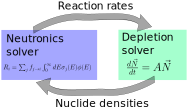
\includegraphics[width=\textwidth]{../images/predictor_diagram.pdf}
\end{frame}

\begin{frame}{Further information}
  \begin{itemize}
    \item OpenMC gives you a
    \href{https://docs.openmc.org/en/latest/pythonapi/deplete.html}{wide choice
    of integrators} with tradeoffs in accuracy, computational cost, and memory
    requirements
    \item For more information on the theoretical background of depletion and
    comparisons of OpenMC with Serpent, see the journal paper by
    \href{https://doi.org/10.1016/j.anucene.2020.107989}{Romano et al.}
  \end{itemize}
\end{frame}

%%---------------------------------------------------------------------------%%

\end{document}
